\section{Transfer of Thermal Energy}

\textbf{Conduction} is the transfer of heat \emph{through a material} from a region of higher temperature to a region of lower temperature.\\
\textbf{Convection} is the transfer of heat \emph{in fluids} due to the movement of material particles of the medium.\\
\textbf{Radiation} is the transfer of heat from one place to another without the use of any material medium.

\begin{multicols}{2}


\subsection{Football Model of Thermal Energy}

\begin{center}
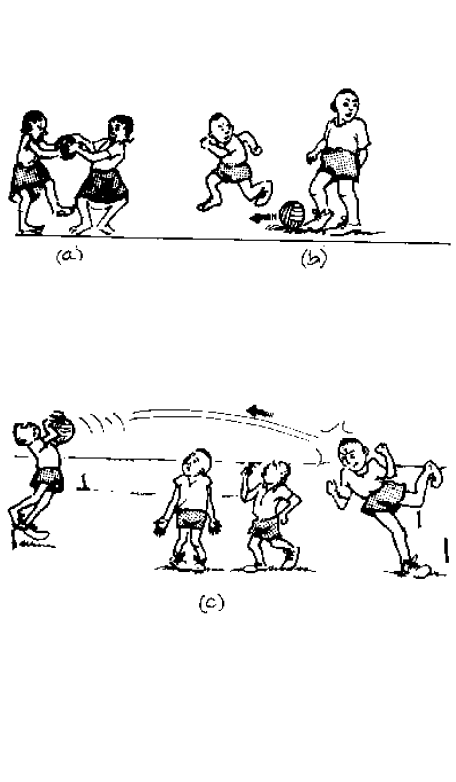
\includegraphics[width=0.49\textwidth]{./img/source/football-thermal.png}
\end{center}

\emph{Conduction} is likened to a football being passed from one player to another, just as heat passes from one molecule to another (a).

\emph{Convection} is likened to a football being taken by one player from one point of the field to another, just as heat in a fluid is transported by a particle from one point to another (b).

\emph{Radiation} is likened to a football being kicked by one player from one point to another without the use of intervening players, just as heat is transmitted from a hot object to another without any medium (c).

\vfill
\columnbreak

\subsection{Heat Transfer in a Candle}

\begin{center}
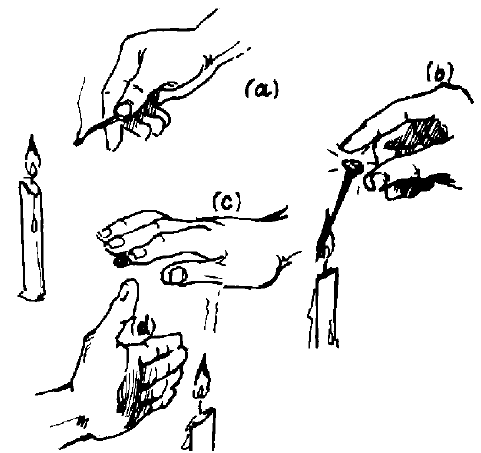
\includegraphics[width=0.49\textwidth]{./img/source/heat-trans-candle.png}
\end{center}

\begin{description*}
%\item[Subtopic:]{}
\item[Materials:]{Candle, nail}
%\item[Setup:]{}
\item[Procedure:]{Light a candle to demonstrate three forms of heat transfer by simple hand movement (a). 

\emph{Conduction}: Stick one end of a nail into the flame (b). 

\emph{Convection}: Place your hand above the flame (c). 

\emph{Radiation}: Place your hand at the side of the flame (d).}
%\item[Hazards:]{}
%\item[Questions:]{}
%\item[Observations:]{In each case heat is transmitted to your hand.}
%\item[Theory:]{}
%\item[Applications:]{}
\item[Notes:]{To see the amount of heat transferred for each case, hold a new matchstick in each arrangement and see how long it takes to ignite the match.}
\end{description*}

\vfill
\columnbreak

%==================================================================================================%

\section*{Conduction}


\subsection{Good and Bad Conductors of Heat}

\begin{center}
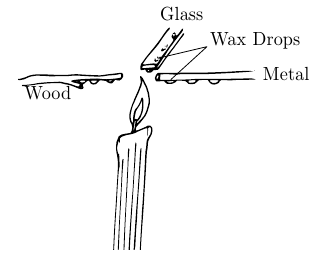
\includegraphics[width=0.4\textwidth]{./img/heat-conduction.png}
\end{center}

\begin{description*}
%\item[Subtopic:]{}
\item[Materials:]{Iron nail, piece of glass, wooden stick, candle, matches}
%\item[Setup:]{}
\item[Procedure:]{Use a lit candle to drip wax at even intervals along the glass, iron and wood (about 1 cm apart). Set the items on the edge of a chair so that one end of each sticks out above the candle (they should not be touching).}
%\item[Hazards:]{}
%\item[Questions:]{}
\item[Observations:]{The wax on the iron nail melts quickly, near the candle first, then moving back along the nail. The wax on the glass melts very slowly while the wax on the stick does not melt at all.}
\item[Theory:]{Heat moves quickly through metal and slowly through wood and glass. Thus metal is a good conductor of heat and glass and wood are poor conductors of heat.}
\item[Applications:]{Cooking pots are made of metal to efficiently transfer heat to the food. \emph{Insulators} are used to prevent heat loss (e.g. in clothes).}
%\item[Notes:]{}
\end{description*}

\subsection{Rate of Conduction}

\begin{center}
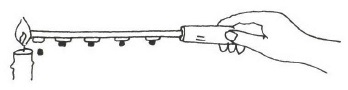
\includegraphics[width=0.45\textwidth]{./img/vso/conduction-rate.jpg}
\end{center}

\begin{description*}
%\item[Subtopic:]{}
\item[Materials:]{Candle, metal rod, small stones or seeds, cloth/paper}
%\item[Setup:]{}
\item[Procedure:]{Use drops of candle wax to stick small stones onto the metal rod at regular intervals. Use a cloth as a handle to hold the end of the rod over the flame.}
%\item[Hazards:]{}
%\item[Questions:]{}
\item[Observations:]{The stones drop off one-by-one along the rod as that part of the rod gets hot.}
\item[Theory:]{The rod conducts heat from the flame, beginning near the flame and then moving back.}
%\item[Applications:]{}
%\item[Notes:]{}
\end{description*}

\subsection{Coin Burn}

\begin{center}
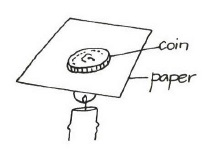
\includegraphics[width=0.35\textwidth]{./img/vso/coin-burn.jpg}
\end{center}

\begin{description*}
%\item[Subtopic:]{}
\item[Materials:]{Coin, paper, candle}
%\item[Setup:]{}
\item[Procedure:]{Place a coin on a piece of paper and hold above a candle so that the coin is directly above the flame.}
%\item[Hazards:]{}
%\item[Questions:]{}
\item[Observations:]{The paper does not burn! Why?}
\item[Theory:]{Metal is a better conductor of heat than paper, so the coin conducts heat away from the candle before the paper burns.}
%\item[Applications:]{}
%\item[Notes:]{}
\end{description*}

\subsection{Paper Pan}

\begin{center}
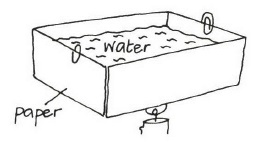
\includegraphics[width=0.4\textwidth]{./img/vso/paper-pan.jpg}
\end{center}

\begin{description*}
%\item[Subtopic:]{}
\item[Materials:]{Paper, paper clips, tape, water, candle}
%\item[Setup:]{}
\item[Procedure:]{Construct a water pan out of paper using paper clips and tape. Fill the pan with water and place over a candle.}
%\item[Hazards:]{}
%\item[Questions:]{}
%\item[Observations:]{}
\item[Theory:]{The paper does not burn as the heat is conducted by the water and the paper never rises above 100$^\circ$C.}
%\item[Applications:]{}
%\item[Notes:]{}
\end{description*}

\subsection{Fireproof Material}

\begin{center}
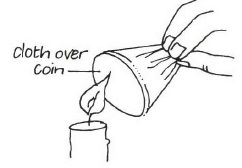
\includegraphics[width=0.4\textwidth]{./img/vso/fireproof.jpg}
\end{center}

\begin{description*}
%\item[Subtopic:]{}
\item[Materials:]{Coin, cloth, candle}
%\item[Setup:]{}
%\item[Procedure:]{}
%\item[Questions:]{}
%\item[Observations:]{}
\item[Theory:]{A coin conducts heat away before the cloth can burn.}
\item[Hazards:]{Do not use synthetic materials as many melt at quite low temperatures.}
%\item[Applications:]{}
%\item[Notes:]{}
\end{description*}

\subsection{Candle Snuffer}

\begin{center}
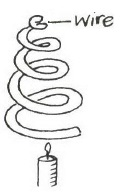
\includegraphics[width=0.2\textwidth]{./img/vso/candle-snuffer.jpg}
\end{center}

\begin{description*}
%\item[Subtopic:]{}
\item[Materials:]{Thick copper wire (about 40 cm), candle}
%\item[Setup:]{}
\item[Procedure:]{Bend the wire into a spiral coil, leaving enough length for a handle. Light a candle and then put out the flame with the snuffer.}
%\item[Hazards:]{}
%\item[Questions:]{}
%\item[Observations:]{}
\item[Theory:]{Copper is a good conductor of heat and thus conducts all of the heat away from the flame.}
%\item[Applications:]{}
%\item[Notes:]{}
\end{description*}

%==================================================================================================%

\section*{Convection}


\subsection{Convection Detectors}

\begin{center}
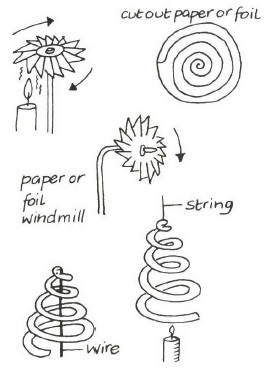
\includegraphics[width=0.49\textwidth]{./img/vso/convection-detectors.jpg}
\end{center}

\begin{description*}
%\item[Subtopic:]{}
%\item[Materials:]{}
%\item[Setup:]{}
\item[Procedure:]{Make the convection detectors shown. If held above a candle they will turn around.}
%\item[Hazards:]{}
%\item[Questions:]{}
%\item[Observations:]{}
%\item[Theory:]{}
%\item[Applications:]{}
%\item[Notes:]{}
\end{description*}

\columnbreak

\subsection{Convection Currents}

\begin{center}
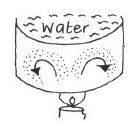
\includegraphics[width=0.25\textwidth]{./img/vso/convection-currents.jpg}
\end{center}

\begin{description*}
%\item[Subtopic:]{}
\item[Materials:]{Clear container/bottle, water, sawdust, candle}
%\item[Setup:]{}
\item[Procedure:]{Fill a container with water and a small amount of sawdust. Heat the container and observe the sawdust.}
%\item[Hazards:]{}
%\item[Questions:]{}
\item[Observations:]{The convection currents are visible in the water.}
\item[Theory:]{The warm water rises and the cooler water sinks down to the bottom as seen by the movement of the sawdust. As the water on top cools, it sinks again to replace the new warm water rising, continuing the cycle.}
\item[Applications:]{Wind, breeze currents}
%\item[Notes:]{}
\end{description*}

\subsection{Breeze as a Convection Current}

\begin{center}
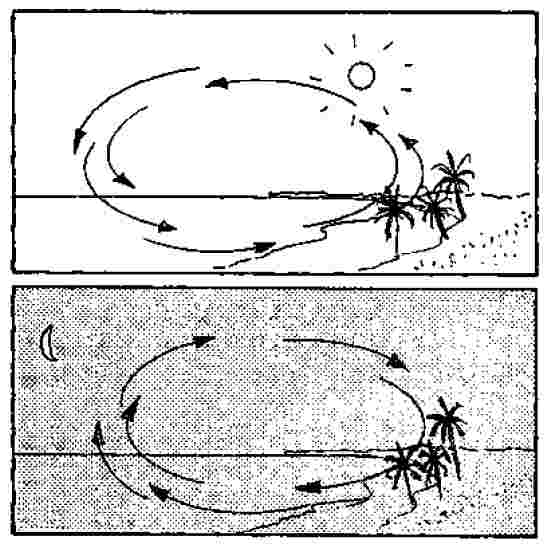
\includegraphics[width=0.4\textwidth]{./img/source/breeze-2.jpg}
\end{center}

\begin{description*}
%\item[Subtopic:]{}
%\item[Materials:]{}
%\item[Setup:]{}
%\item[Procedure:]{}
%\item[Hazards:]{}
%\item[Questions:]{}
\item[Observations:]{At the coast and on lake shores, a gentle air stream or \emph{breeze} is always blowing. The direction of the breeze during the day is different from that at night.}
\item[Theory:]{During daytime, the land warms up faster than the sea. The warm air rises over the land and cooler air from the sea flows to the land. This creates a breeze from sea to land.

During night, the water stays warmer than the land, air over the water rises, colder air from the land flows to the sea. This creates a breeze from land to sea.}
%\item[Applications:]{}
%\item[Notes:]{}
\end{description*}

\columnbreak

\subsection{Ventilation System}

\begin{center}
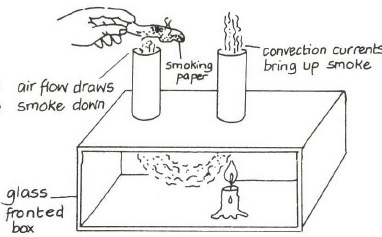
\includegraphics[width=0.45\textwidth]{./img/vso/ventilation-system.jpg}
\end{center}

\begin{description*}
%\item[Subtopic:]{}
\item[Materials:]{Glass- or plastic-fronted box, 2 cardboard tubes, candle, smoking paper}
\item[Setup:]{Make 2 holes in the top of the box and push in the cardboard tubes. Place a candle under one of the tubes.}
\item[Procedure:]{Light the candle and hold a smoking cloth or paper above the other tube.}
%\item[Hazards:]{}
%\item[Questions:]{}
\item[Observations:]{Smoke is drawn into the first tube and flows out the other.}
\item[Theory:]{Convection currents can be seen by the movement of the smoke. The air heated by the candle rises, allowing for cooler smoky air to flow downward through the first tube. As this air is heated, it then moves upward out of the second tube.}
\item[Applications:]{Ventilating a room, drawing in cool air to a container}
%\item[Notes:]{}
\end{description*}

\subsection{Hot Air Balloon}

\begin{center}
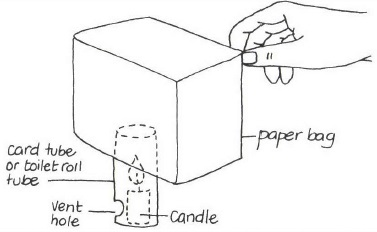
\includegraphics[width=0.45\textwidth]{./img/vso/hot-air-balloon.jpg}
\end{center}

\begin{description*}
%\item[Subtopic:]{}
\item[Materials:]{Lightweight paper bag, candle, cardboard tube}
\item[Setup:]{Cut a small vent hold at the bottom of a toilet paper tube and place a candle inside the tube.}
\item[Procedure:]{Light the candle and hold the bag over it.}
%\item[Hazards:]{}
%\item[Questions:]{}
\item[Observations:]{The bag rises as the air inside heats up.}
\item[Theory:]{Warm air is lighter than cool air, so it rises upward. If the bag is light enough, it will be lifted by the air current.}
\item[Applications:]{Have students design their own hot air balloons and test which flies highest.}
%\item[Notes:]{}
\end{description*}

%==================================================================================================%

\section*{Radiation}


\subsection{Good and Bad Radiators}

\begin{center}
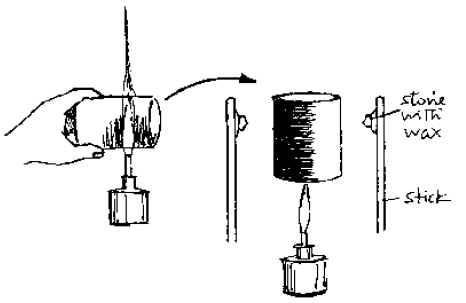
\includegraphics[width=0.4\textwidth]{./img/source/good-bad-radiators.png}
\end{center}

\begin{description*}
%\item[Subtopic:]{}
\item[Materials:]{Shiny can, black paint/shoe polish, 2 wooden sticks, candle, 2 small stones}
\item[Setup:]{Paint one half of the outside of an open can or cover with soot by holding over a candle. Leave the other half shiny.}
\item[Procedure:]{Place a wooden stick near each side of the can. Stick a small stone with candle wax on each stick. Heat the bottom of the can.}
%\item[Hazards:]{}
%\item[Questions:]{}
\item[Observations:]{The candle wax opposite the blackened surface begins to melt faster than the wax opposite the shiny surface.}
\item[Theory:]{A black surface is a better radiator than a shiny surface.}
%\item[Applications:]{}
%\item[Notes:]{}
\end{description*}

\subsection{Good and Bad Heat Absorbers}

\begin{center}
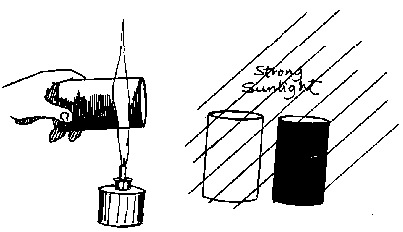
\includegraphics[width=0.4\textwidth]{./img/source/good-bad-absorbers.png}
\end{center}

\begin{description*}
%\item[Subtopic:]{}
\item[Materials:]{2 identical cans, black paint/shoe polish, candle}
\item[Setup:]{Paint the outside of one can black or cover with soot by holding it over a candle.}
\item[Procedure:]{Place both cans in the sun or at equal distances from a fire for about a half hour. Then feel each can.}
%\item[Hazards:]{}
\item[Observations:]{The blackened can is hotter than the shiny can.}
\item[Theory:]{A black surface absorbs heat more quickly than a shiny surface.}
\item[Applications:]{It is wise for people in hot areas to wear bright clothes and paint their houses white so that they absorb less heat.}
\item[Questions:]{What colour should a petrol tank be painted? Why?}
%\item[Notes:]{}
\end{description*}

%==================================================================================================%


\end{multicols}

\pagebreak